\begin{problem}{All Satisfying Assignments}
Consider a modified CSP in which we wish to find every possible satisfying assignment, rather than just one such assignment as in normal CSPs. In order to solve this new problem, consider a new algorithm which is the same as the normal backtracking search algorithm, except that when it sees a solution, instead of returning it, the solution gets added to a list, and the algorithm backtracks. Once there are no variables remaining to backtrack on, the algorithm returns the list of solutions it has found.\\\\
For each graph below, select whether or not using the MRV and/or LCV heuristics could affect the number of nodes expanded in the search tree in this new situation.

\begin{question}[8]{}\\
\begin{tabular}{cl}
&\\
\multirow{1}{*}{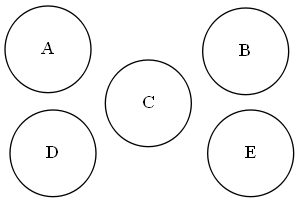
\includegraphics[scale=0.5]{figures/disconnected.png} \hspace{1.4in}} &
\AnswerThreeA
\end{tabular}\\
\end{question}

\vspace{-.2in}
\begin{question}[8]{}\\
\begin{tabular}{cl}
\multirow{1}{*}{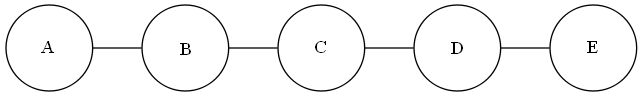
\includegraphics[width=3in]{figures/chain.png}} &
\AnswerThreeB
\end{tabular}\\
\end{question}

\vspace{-.2in}
\begin{question}[8]{}\\
\begin{tabular}{cl}
\multirow{1}{*}{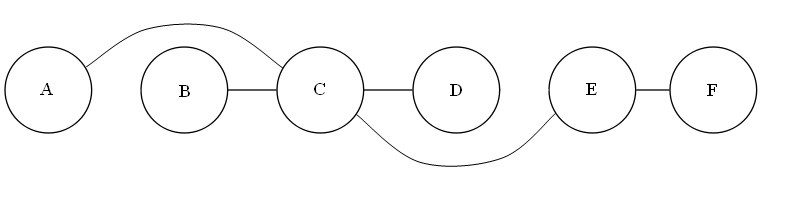
\includegraphics[width=3in]{figures/tree.png}} &
\AnswerThreeC
\end{tabular}
\end{question}

\vspace{-.2in}
\begin{question}[8]{}\\
\begin{tabular}{cl}
\multirow{1}{*}{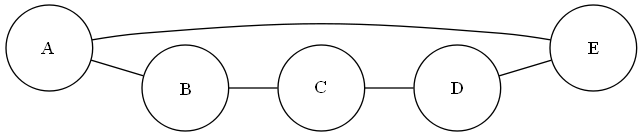
\includegraphics[width=3in]{figures/circle.png}} &
\AnswerThreeD
\end{tabular}
\end{question}

\vspace{-.2in}
\begin{question}[8]{}\\
\begin{tabular}{cl}
\multirow{1}{*}{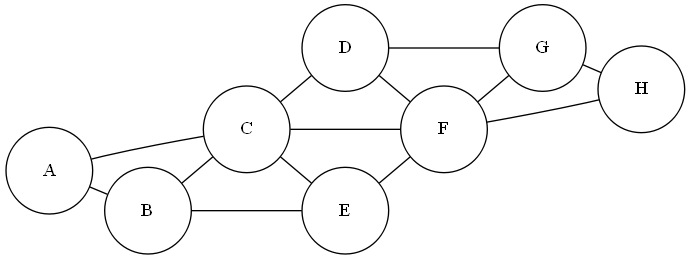
\includegraphics[width=3in]{figures/csp_graph.png}} &
\AnswerThreeE
\end{tabular}
\end{question}

\end{problem}